\documentclass[tikz, border=2pt]{standalone}

\usepackage{tikz}
\usetikzlibrary{calc}
\usepackage{drawstack}

\begin{document}

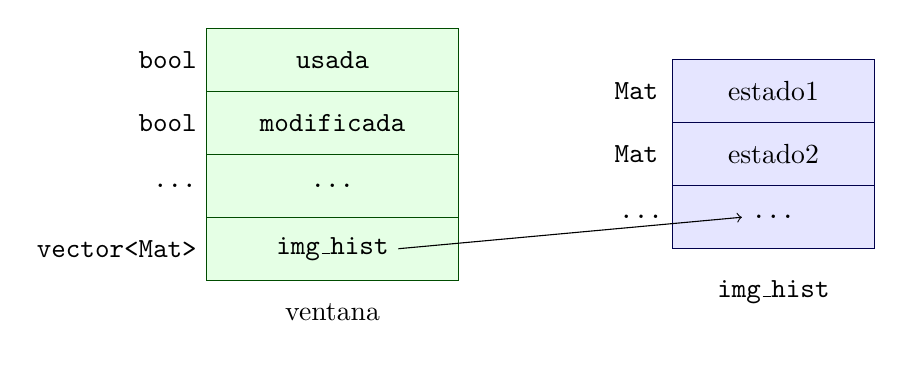
\begin{tikzpicture}[scale=0.8]

  \cell{\texttt{usada}}        \cellcomL{\texttt{bool}}     \coordinate (usada) at (currentcell.east);
  \cell{\texttt{modificada}}   \cellcomL{\texttt{bool}}     \coordinate (modificada) at (currentcell.east);
  \cell{\texttt{...}}          \cellcomL{\texttt{...}}
  \cell{\texttt{img\_hist}}    \cellcomL{\texttt{vector<Mat>}} \coordinate (ih) at (currentcell.east);
  \cell[draw=none]{ventana}

  \drawstruct{(7,-0.5)}
  \structcell{estado1}
  \node[anchor=east] at ($(currentcell.west)+(-0.8,0)$) {\texttt{Mat}};
  \structcell{estado2}
  \node[anchor=east] at ($(currentcell.west)+(-0.8,0)$) {\texttt{Mat}};
  \structcell{\texttt{...}}
  \node[anchor=east] at ($(currentcell.west)+(-1.1,0)$) {\texttt{...}};
  \node at ($(currentcell.south)+(0,-1)$) {\texttt{img\_hist}};
  \coordinate (IHnode) at (currentcell.west);
  \coordinate (IHanchor) at (currentcell.south);

  \draw[->] (ih) -- (IHnode);

\end{tikzpicture}

\end{document}

